\chapter{Introduction}
\newcommand{\doublemu}{ \vec{\mu} \boldsymbol{\mu}  }

As a young graduate student, I was incredibly disappointed by the resources available to me to learn the physics about what is going on in electronic spectroscopy.  Thus, I am going to use the opportunity here to attempt to write a useful and pedagogical introduction to the physics behind Electronic Spectroscopy in the hopes that future students can hit the ground running faster than I was able to.

\section{Electric Field Interactions with Quantum Systems}
Let's imagine that we have in our possession a two-level Quantum System with a Hamiltonian like so:
\begin{align}
	H = \left( \begin{array}{ccc}
		0 & 0 \\
		0 & E_1 \end{array} \right)
\end{align}
We don't have to assume a two level system and indeed, most of the time we won't know the exact nature of the system before we begin the experiment.  For the purposes of explaining what's going on, however, the two level system more than suffices and is much easier to type (for me) and write (for you) so we will stick with it for now.

Anyway, we have decided that we want to see what happens when we hit this guy with light.  Why?  What are we going to learn?

\subsection{What are we trying to learn?}
When we hit the system with light, we can learn about the structure of the system and the dynamics of how that structure evolves.

This happens because when the system is excited with light, it will, itself, emit light.  The light that comes forth from our system will encode very basic information about the system and out theory here can predict what it will say.

\subsection{What is physically going on?}
We have in our possession a femtosecond laser which can output electric fields of the following Gaussian form:
\begin{align}
	\vec{E}(t) = \vec{\textbf{e}} \frac{A}{\sqrt{2 \pi \sigma^2}} e^{-(t - T)^2 / 2 \sigma^2} \left( e^{i \vec{k} \cdot \vec{r} - i \omega_c t + i\phi}  + e^{-i \vec{k} \cdot \vec{r} + i \omega_c t - i\phi} \right)
\end{align}
Where the parameters are as follows:
\begin{center}
\begin{tabular}{l | l}
	$\vec{\textbf{e}}$ & the polarization and of the beam \\
	$\sigma$ & spread parameter of the beam in time \\
	$ \omega_c$ & the frequency of the carrier wave \\
	$\vec{k}$ & the wave-vector of the beam\\
	$T$ & the center-time of the pulse \\
	$\phi$ & the phase of the pulse
\end{tabular}
\end{center}
What's that you say?  The magnetic field?  We're going to assume it's negligible since $|B| \propto |E| / c$ and $c$ is generally assumable to be a big number.

You may be rightfully asking at this point: how is this electric field going to interact with our quantum system?  For that answer, we must appeal to electrodynamics and, specifically, the electrodynamic quantum mechanical Hamiltonian (which we will refrain from deriving or otherwise generating).
\begin{align}
	H = \sum_i \frac{\left|  \vec{p_i} - \frac{q_i}{c} \vec{A}(\vec{r_i}, t)  \right|^2}{2 m_i} + q_i \phi(\vec{r_i}, t)
\end{align}
Where the sum is over all particles in the system.  Theoretically, this is all we need to begin simulations.  Just define a vector potential for the input field and then a vector and scalar potential for the system and you're done.

Unfortunately, that's not going to work.  While in theory a simulation like that is possible, the scaling would be awful and even with a modern supercomputer, there's not way we could treat anything more than a small system.  Furthermore, we were talking about our system in terms of energy states, not particles, so we need to find a way to get this Hamiltonian to look like it will play well with energy states.  To do this, let's expand out the Hamiltonian.
\begin{align}
	H = \sum_i \left[ \frac{\vec{p}_i^2}{2 m_i} + q_i \phi(\vec{r_i}, t) \right] - \frac{q_i}{2 m c} \left(\vec{p}_i \cdot \vec{A}(\vec{r_i}, t) +  \vec{A}(\vec{r_i}, t)\cdot \vec{p}_i \right) + \frac{q_i^2 }{2 m_i c^2} \vec{A}(\vec{r_i}, t)^2
\end{align}
Let's now assume that we're in the Coulomb gauge and the following are true:
\begin{eqnarray}
	\nabla \cdot \vec{A} = 0 \\
	\vec{E} = -\frac{\partial \vec{A}}{\partial t} \\
	\vec{B} = \nabla \times \vec{A}
\end{eqnarray}
Since the momentum operator is the gradient, that gives us our first simplification:
\begin{align}
	H = \sum_i \left[ \frac{\vec{p}_i^2}{2 m_i} + q_i \phi(\vec{r_i}, t) \right] - \frac{q_i}{2 m c} \vec{A}(\vec{r_i}, t)\cdot \vec{p}_i  + \frac{q_i^2 }{2 m_i c^2} \vec{A}(\vec{r_i}, t)^2
\end{align}
Now the trick we want here is to make yet another gauge transformation like so:
\begin{align}
	f &= \vec{A}\cdot \vec{r} \\
\end{align}
Which will affect $\vec{A}$ like so
\begin{align*}
	\vec{A} &\rightarrow \vec{A} + \nabla f \\
			&=\vec{A} + \nabla \cdot \vec{A} \\
	\nabla \left(  \vec{A}\cdot \vec{r}  \right) &= \vec{A} \times (\nabla \times \vec{r}) + \vec{r}\times (\nabla \times \vec{A} ) + (\vec{A} \cdot \nabla ) \vec{r} + (\vec{r} \cdot \nabla )\vec{A} \\
	&= \vec{r}\times \vec{B} + \vec{A} + (\vec{r} \cdot \nabla )\vec{A} \\
	\vec{A} &\rightarrow 2\vec{A} + \vec{r}\times \vec{B}  + (\vec{r} \cdot \nabla )\vec{A}
\end{align*}
and $\phi$ like so:
\begin{align*}
	\phi &\rightarrow \phi -\frac{\partial}{\partial t} f \\
	&\rightarrow \phi -\frac{\partial}{\partial t} \vec{A}\cdot \vec{r} \\
	&\rightarrow \phi + \vec{E} \cdot \vec{r}
\end{align*}
Alright, now the electric field appears.  Going back to the Hamiltonian:
\begin{align*}
	H &= \sum_i \left[ \frac{\vec{p}_i^2}{2 m_i} + q_i \phi(\vec{r_i}, t) \right] \\
	  &+ q_i \vec{E}(t, \vec{r}_i) \cdot \vec{r_i} \\
	  &- \frac{q_i}{2 m c} \left( 2 \vec{A}(\vec{r_i}, t) +  \vec{r}_i \times \vec{B}(\vec{r_i}, t)  + \vec{r}_i \cdot \nabla_i \right)\cdot \vec{p}_i  \\
	  &+ \frac{q_i^2 }{2 m_i c^2} \left( 2 \vec{A}(\vec{r_i}, t) +  \vec{r}_i \times \vec{B}(\vec{r_i}, t)  + \vec{r}_i \cdot \nabla_i \right)^2
\end{align*}
This looks workable, does it not?  OK, so given that in molecular systems, the Hamiltonian is just a collection of Coulomb terms with no time dependence, we will say that the first line of the above equation is the system Hamiltonian and all the time dependence of $\phi$ is just manifest in the Electric field of the incoming light.

We now make the famous \textbf{Electric Dipole Approximation} which basically says that since $c$ is large, the only term that matters in the above expression is the Electric field.  Why do we call is the electric dipole approximation?  Because it involves the dipole operator:
\begin{align*}
	H'(t) &=  \sum_i q_i \vec{E}(t, \vec{r}_i) \cdot \vec{r_i} \\
\end{align*}
Which, if we assume the electric field is constant across all the particles in the system (another big part of the electric dipole approximation), we can calculate matrix elements,
\begin{align*}
	H_{ab}'(t) &= \vec{E}(t, \vec{r}) \cdot \bra{a} \sum_i q_i  \vec{r_i} \ket{b}\\
\end{align*}
\begin{align}
	H_{ab}'(t) &= \vec{E}(t, \vec{r}) \cdot \vec{\mu}_{ab}
\end{align}
We now have a way of describing the interaction of light with an electronic system.
\subsection{The Dipole Matrix}
The dipole matrix we have just derived is a very useful thing.  The first claim I want to make is that it is a completely off-diagonal matrix.
\subsubsection{Off-Diagonal}
To explain this, let's go to one dimension and assume some position space form for the energy eigenfunctions of the system:
\begin{align}
	\mu_{aa} = \int_{-\infty}^{\infty} a^{\dagger}(x) x a(x) dx
\end{align}
If the claim is that this is equal to zero, I can prove this simply by proving that $a^{\dagger}(-x) -x a(-x) = -a^{\dagger}(x) x a(x)$ which is equivalent  to determining $a^{\dagger}(-x) a(-x) = a^{\dagger}(x) a(x)$ because of our friend the $x$ operator.  This itself is equivalent to determining that the function for $a$ and its hermitian conjugate have the same parity ($\pm$ behavior under coordinate mirroring).
\begin{align}
	a^{\dagger}(-x)  &= \pm a^{\dagger}(x)  \\
	a(-x) &= \pm a(x)
\end{align}
To do this, let's assume that they have the opposite behavior:
\begin{align}
	a^{\dagger}(-x)  &= - a^{\dagger}(x)  \\
	a(-x) &=  a(x)
\end{align}
And try to normalize the wavefunction
\begin{align}
	1 &= \int_{-\infty}^{\infty} a^{\dagger}(x) a(x) dx \\
		&= \int_{-\infty}^{0} a^{\dagger}(x) a(x) dx + \int_{0}^{\infty} a^{\dagger}(x) a(x) dx \\
		&= -\int_{\infty}^{0} a^{\dagger}(-x) a(-x) dx + \int_{0}^{\infty} a^{\dagger}(x) a(x) dx \\
		&= -\int_{0}^{\infty} a^{\dagger}(x) a(x) dx + \int_{0}^{\infty} a^{\dagger}(x) a(x) dx  = 0
\end{align}
Clearly then, our original assumption is false and they have the same parity behavior and the dipole matrix is off-diagonal

\subsubsection{Physical Meaning of the Dipole Matrix}
But what does the Dipole Matrix represent?  To understand this, let's look at the matrix representation:
\begin{align}
	\vec{\mu} = \left( \begin{array}{ccc}
		0 & \vec{\mu}_{01} \\
		\vec{\mu}_{10} & 0 \end{array} \right)
\end{align}
Let's imagine a wavefunction in the ground state:
\begin{align}
	\ket{\Psi} = \left( \begin{array}{ccc}
		1 \\
		0 \end{array} \right)
\end{align}
What happens when we act the dipole operator on the wavefunction?
\begin{align}
	\vec{\mu} \ket{\Psi} &= \left( \begin{array}{ccc}
		0 & \vec{\mu}_{01} \\
		\vec{\mu}_{10} & 0 \end{array} \right)
	\left( \begin{array}{ccc}
		1 \\
		0 \end{array} \right) \\
	 &= \left( \begin{array}{ccc}
		0 \\
		\vec{\mu}_{10} \end{array} \right)
\end{align}
It induces a transition from the ground state to the excited state, which corresponds to the Absorption of a photon.  It is for this reason that it is sometimes called the ``Transition Dipole Operator''.  Just for fun, let's act it on the excited state as well.
\begin{align}
	\ket{\Psi} &= \left( \begin{array}{ccc}
		0 \\
		1 \end{array} \right) \\
	\vec{\mu} \ket{\Psi} &= \left( \begin{array}{ccc}
		0 & \vec{\mu}_{01} \\
		\vec{\mu}_{10} & 0 \end{array} \right)
	\left( \begin{array}{ccc}
		0 \\
		1 \end{array} \right) \\
	 &= \left( \begin{array}{ccc}
		\vec{\mu}_{01} \\
		 0 \end{array} \right)
\end{align}
It just brought it down to the excited state.  This corresponds to the ``Stimulated Emission'' of a photon.  Given that this operator induces transition, the following notation makes it easier to understand what's going on:
\begin{align}
	\vec{\mu} = \left( \begin{array}{ccc}
		0 & \vec{\mu}_{0 \leftarrow 1} \\
		\vec{\mu}_{1 \leftarrow 0} & 0 \end{array} \right)
\end{align}

\subsubsection{Transition Dipole Matrix Notation}
The transition Dipole Matrix has a dual role as an operator and a vector in space.  Which makes the notation of $\vec{\mu}$ seem incomplete.  Therefore, I propose the following notation instead:
\begin{align}
	\doublemu = \left( \begin{array}{ccc}
		0 & \vec{\mu}_{0 \leftarrow 1} \\
		\vec{\mu}_{1 \leftarrow 0} & 0 \end{array} \right)
\end{align}
Pronounced ``Double-mu'' for hopefully obvious reasons, each 'mu' represents a part of the nature of the object: either operator or vector.  I hope you will like it.

Furthermore, there may also come a day when we need a non-matrix representation of the dipole operator for convenience's sake.
\begin{align}
	\doublemu = \sum_{i \neq j} \vec{\mu}_{j \leftarrow i} \ket{j} \bra{i}
\end{align}


\subsection{Putting it all together}
After some algebra we can now go back to the physics of the situation.  Recall that we're dealing with a two-level system like this:

\begin{align}
	H = \left( \begin{array}{ccc}
		0 & 0 \\
		0 & E_1 \end{array} \right)
\end{align}
And now we have a Hamiltonian which describes how this system interacts with radiation:
\begin{align}
	H'(t) = \vec{E}(r, t) \cdot \doublemu
\end{align}
\begin{align}
	\vec{E}(\vec{r}, t) = \vec{\textbf{e}} \frac{A}{\sqrt{2 \pi \sigma^2}} e^{-(t - T)^2 / 2 \sigma^2} \left( e^{i \vec{k} \cdot \vec{r} - i \omega_c t - i \phi}  + e^{-i \vec{k} \cdot \vec{r} + i \omega_c t - i \phi} \right)
\end{align}

We now know fully how light interacts with a quantum system but only at a very high level of the Hamiltonian.  We just have this weird object which we know nothing about how to manipulate yet.  Furthermore, how does this system emit light?  First let's tackle how to incorporate this Hamiltonian into a wavefunction.






\section{Time-Dependent Quantum Mechanics}

With any Hamiltonian you can just go about solving the  Quantum-Mechanical differential equation
\begin{align*}
	\frac{d}{dt} \Ket{\Psi(t)}  = - \frac{i}{\hbar} H \Ket{\Psi(t)}
\end{align*}
in any way you desire.  If $H$ is time-independent and you can precisely identify the wavefunction at an initial time $t_0$, this is super easy since you just solve a dead-simple differential equation to get:

\begin{align*}
	\Ket{\Psi (t)}  = e^{- \frac{i}{\hbar} H_0 (t - t_0)} \Ket{\Psi(t_0)}  \\
	\Ket{\Psi (t)}  = U(t, t_0) \Ket{\Psi(t_0)}
\end{align*}
Where $U(t, t_0)$ is the ``Time-Evolution Operator''.

We can not, however, do something quite this simple for a generalized time-dependent Hamiltonian

\section{Perturbation Treatment}
To treat a time-dependent Hamiltonian, we have to go back to the initial equation:

\begin{align*}
	\frac{d}{dt} \Ket{\Psi(t)}  = - \frac{i}{\hbar} H(t) \Ket{\Psi(t)}
\end{align*}
Rearrange it to get the beginning of the solution to the differential equation:
\begin{align*}
	d \Ket{\Psi(t)}  = - \frac{i}{\hbar} H(t)  \Ket{\Psi(t)} dt
\end{align*}
Now let's integrate both sides from $t_0$ to a general time $t$:
\begin{align*}
	\Ket{\Psi(t)} - \Ket{\Psi(t_0)}  &= - \frac{i}{\hbar} \int_{t_0}^{t} H(\tau)  \Ket{\Psi(\tau)} d\tau \\
	\Ket{\Psi(t)} & = \Ket{\Psi(t_0)} - \frac{i}{\hbar} \int_{t_0}^{t} H(\tau)  \Ket{\Psi(\tau)} d\tau
\end{align*}
And there we have solved it ... Oh wait, shoot, this equation is self-referential.  No matter, we'll just plug it in again,

\begin{align*}
	\Ket{\Psi(t)} & = \Ket{\Psi(t_0)} - \frac{i}{\hbar} \int_{t_0}^{t} H(\tau)  \Ket{\Psi(t_0)} d\tau + \left( \frac{i}{\hbar}\right)^2 \int_{t_0}^{t} H(\tau) \int_{t_0}^{\tau}  H(\tau')  \Ket{\Psi(\tau')} d\tau' d\tau
\end{align*}
Since this seems to be going on for infinity (spoiler alert: it is), it seems best to define then a series of wavefunctions like so:
\begin{align}
	\Ket{\Psi(t)} &= \sum_{i} \Ket{\Psi^{(i)} (t)} \\
	\Ket{\Psi^{(0)} (t)} &= \Ket{\Psi(t_0)} \\
	\Ket{\Psi^{(n)} (t)} &= - \frac{i}{\hbar} \int_{t_0}^{t} H(\tau)  \Ket{\Psi^{(n-1)} (\tau)} d\tau
\end{align}
What is happening here?  The first perturbation term is the Hamiltonian acting on the system once.  In our case, it's almost always a photon so what is happening, here, is the first order term is one photon interacting, the second two photons etc.

The integral, it will soon become clear, is taking every time that the light beam is ``on'' and could interact with the system once, and interfering together, all the possible times that the interaction could happen.  This is more clear, ironically, when we shift around these equations into what is called the  ''interaction picture'':

\subsubsection{The Interaction Picture}

The perturbation integrals are probably going to be rather difficult to calculate and, since the integrand is never going to equal zero, we won't be able to cut any corners to save time.  You will recall, however, that the Gaussian pulses we are looking to hit our system with do approach zero.  For that reason, let's start by splitting the Hamiltonian into a time-independent and time-dependent part:
\begin{align}
	H(t) = H_0 + H'(t)
\end{align}
For the time-independent part, we know we can define the propagator $U_0(t, t_0) = e^{-i (t - t_0) H_0 / \hbar}$ which is how the system evolves in time if there is no time-dependent interaction term.  Note that because this is merely the evolution when there is not time-dependent perturbation, if we are working in a density matrix formalism, this could easily include dephasing.

To spare an awkward derivation I'll cut right to the chase: for any operator and for the actual, true wavefunction, we define the ``interaction'' operator and wavefunctions:
\begin{align}
	\Ket{\Psi_I(t)} = U_0^{\dagger}(t, t_0) \Ket{\Psi(t)} \\
	A_I(t) = U_0^{\dagger}(t, t_0) A(t) U_0(t, t_0)
\end{align}
Why did we do that?  Just wait, all will be revealed.  I will leave it up to you to confirm that:
\begin{align}
	\frac{d}{dt} \Ket{\Psi_I(t)} = \frac{i}{\hbar} H_I (t) \Ket{\Psi_I(t)}
\end{align}
Huh, OK so that means that our perturbation series stays the same as well with the addition of $I$ subscripts:
\begin{align}
	\Ket{\Psi_I(t)} &= \sum_{i} \Ket{\Psi_I^{(i)} (t)} \\
	\Ket{\Psi_I^{(0)} (t)} &= \Ket{\Psi_I(t_0)} \\
	\Ket{\Psi_I^{(n)} (t)} &= - \frac{i}{\hbar} \int_{t_0}^{t} H'_I(\tau)  \Ket{\Psi_I^{(n-1)} (\tau)} d\tau
\end{align}
Let's begin by examining the zero order term and bringing it back into the actual wavefunction picture:
\begin{align}
	\Ket{\Psi_I^{(0)} (t)} &= \Ket{\Psi_I(t_0)} \\
	U_0^{\dagger}(t, t_0)\Ket{\Psi^{(0)} (t)} &= U_0^{\dagger}(t_0, t_0) \Ket{\Psi(t_0)} \\
	\Ket{\Psi^{(0)} (t)} &= U_0(t, t_0) \Ket{\Psi(t_0)}
\end{align}
This means that after our interaction picture transformation, zero-order estimate for the wavefunction's evolution is just how the wavefunction would evolve without a perturbation, which hopefully makes a lot of sense. Now let's look at the first order correction:

\begin{align}
	U_0^{\dagger}(t, t_0)\Ket{\Psi^{(1)} (t)} &= - \frac{i}{\hbar} \int_{t_0}^{t} U_0^{\dagger}(\tau, t_0) H'(\tau) U_0(\tau, t_0)  \Ket{\Psi^{(0)}(t_0)} d\tau \\
	\Ket{\Psi^{(1)} (t)} &=- \frac{i}{\hbar} \int_{t_0}^{t} U_0(t, \tau) H'(\tau)  \Ket{\Psi^{(0)}(\tau)} d\tau
\end{align}

Here we have the system evolving, minding its own business until time $\tau$ when it decides to interact with the perturbation which in this case is also interacting with a photon: absorbing or emitting.  After it has interacting with the photon, it goes again on its merry way, evolving in time without the perturbation.  The system can 'decide' to interact with a photon at any time the perturbation is 'on', so the integral serves to average over all possible time the photon can interact with the system.

It should further be clear that the 0th order correction is 0 photons interacting with the system, the first order is one photon, second two photons, ad nauseum.  So from now on, we take the interaction picture derivation as moot and use the following equations to do all of our time-dependent Quantum Mechanics:

\begin{align}
   \ket{\Psi_0 (t)} &= U_{0} (t, t_0) \ket{\Psi(t_0)} \\
   \ket{\Psi^{(n)} (t)} &= -\frac{i}{\hbar} \int_{t_0}^{t} \hat{H} (\tau) \ket{\Psi^{(n-1)} (\tau)} d\tau
\end{align}



\subsubsection{Multiple Hamiltonians}
Whenever you can express the perturbation Hamiltonian as a sum of other Hamiltonians (like in a multiple laser beam spectroscopy experiment), you may want to talk about applying them in a certain order in which case the above notation is far too simplistic,
\begin{align}
	H'(t) &= \hat{H}'_1(t) + \hat{H}'_2(t) + \hat{H}'_3(t) \\
	\ket{\Psi_{1}(t)} &= -\frac{i}{\hbar} \int_{t_0}^{t} \hat{H}_1 (\tau) \ket{\Psi_0 (\tau)} d\tau\\
	\ket{\Psi_{1,2}(t)} &= -\frac{i}{\hbar} \int_{t_0}^{t} \hat{H}_2 (\tau) \ket{\Psi_{1} (\tau)} d\tau
\end{align}
Where the interactions can be read from left to right.  So for example, that last equation represents one interaction of the first perturbation, followed by another interaction of the second Hamiltonian



\section{Electric Field Emissions from Quantum Systems}
We're still missing a huge piece, though.  Sure, we could now go on to calculate how the wavefunction evolves in time... but how   we measure this?  Fear not, for our savior comes in the form of the dipole operator.  Recall from your Electricity and Magnetism courses that an oscillating dipole will produce radiation.  So let's plan on doing that: on taking the time-expectation value of the dipole operator:

\begin{align}
	\vec{D}_i(t) &= \Bra{\Psi(t)} \doublemu \Ket{\Psi(t)}
\end{align}
That is for the dipole on one molecule or one system.  For multiple systems, you sum the dipoles together to get the macroscopic ``Polarization''.  For our General case, we use Mukamel~\cite{Mukamel1995} Equation 4.75 but ignore the term for phase matching, assuming that it's always fulfilled for the systems we will treat.
\begin{align}
	\vec{E}_{\text{emission}}(t) = i \frac{2 \pi}{n(\omega_s)} \frac{\omega_s}{c} l P(t) = i \sum_j D_{j}(t)
\end{align}
This number is actually dimensionless so in the interest of accuracy, we want to know what the prefactor is.  According to Griffith's~\cite{GriffithsEM}, the form of the electric field for a simple oscillating dipole (form given below) and far away from the source is:
\begin{align}
	\vec{p}(t) &= q_0 d \hat{z} \cos \omega t = \vec{p}_0 \cos \omega t \\
	\vec{E}(t) &= -\frac{p_0}{4 \pi \epsilon_0} \frac{\omega^2}{c^2} \cos \omega \left( t - \frac{r}{c} \right) \left(\hat{r} \cos \theta - \hat{z} \right)
\end{align}
The prefactor constants are not terribly important for our purposes, but the  $\omega^2$ could very important as it will be different for different signals.  Generally, however, we can ignore it, except in some cases, especially where I compare to experiment.  So I will then take a hybrid approach in those cases where we keep the imaginary factor as it is a result of Quantum Mechanics but establish the pre-factor of $\frac{1}{4 \pi \epsilon_0} \frac{\omega^2}{c^2}$.  The factor $r/c$ retarding the dipole does not concern us here, neither does the direction of the dipole.  The direction would also matter if we were investigating systems where there were multiple dipoles at different directions, but we do not have that in any of the systems of interest in this thesis.

% \textbf{I would like to be able to repeat Mukamel's derivation as it is truly the last bit of science that I don't 100\% understand in my project, but I'm putting this as a todo for the time being, that I only might get back to:}
% TODO: DERIVE the output electric field in terms of polarization

\subsection{What is Actually Being Measured}
Imagine you have an input pulse $\vec{E}_{\text{in}}(t)$ and then some molecular output $\vec{E}_{\text{out}}(t)$.  Most detectors actually detect the intensity of light which is the mod squared of the electric field.  So that detector is actually measuring:
\begin{align}
	I_{\text{total}}(t) &= \left| \vec{E}_{\text{in}}(t) + \vec{E}_{\text{out}}(t) \right|^2 \\
	&= \left( \vec{E}_{\text{in}}(t) + \vec{E}_{\text{out}}(t) \right) \left( \vec{E}_{\text{in}}(t) + \vec{E}_{\text{out}}(t) \right)^*\\
	&= I_{\text{in}}(t) + I_{\text{out}}(t) + \vec{E}^*_{\text{out}}(t) \cdot  \vec{E}_{\text{in}}(t) +  \vec{E}_{\text{out}}(t) \cdot \vec{E}^*_{\text{in}}(t)
\end{align}
We now have a simple complex number arithmetic problem in from of us
\begin{align*}
	\textbf{a} &= a_r + i a_i \\
	\textbf{b} &= b_r + i b_i \\
	\textbf{a} \textbf{b}^* &= a_r b_r + a_i b_i + i(-a_r b_i + a_i b_r)\\
	\textbf{a}^* \textbf{b} &= a_r b_r + a_i b_i + i(a_r b_i - a_i b_r) \\
	\textbf{a} \textbf{b}^* + \textbf{a}^* \textbf{b} &= 2 \left( a_r b_r + a_i b_i\right) \\
	\textbf{a} \textbf{b}^* + \textbf{a}^* \textbf{b} &= 2 \text{Re}\left[ \textbf{a} \textbf{b}^*  \right]= 2 \text{Re}\left[ \textbf{a}^* \textbf{b}   \right]
\end{align*}
which bringing it back:
\begin{align}
	I_{\text{total}}(t) &= I_{\text{in}}(t) + I_{\text{out}}(t) +  2 \text{Re}\left[ \vec{E}_{\text{out}}(t) \cdot \vec{E}^*_{\text{in}}(t)\right]
\end{align}
OK, so there first term here is big (we are using a laser after all) and most likely known (although not necessarily always).  Then the second term is interesting but is going to be much smaller then the next term which describes the interference between the input pulse and the output emission.  This third term will be what we measure most of the time, since it provides a way to make it easier to measure the small signal we care about, since it's attached to a large signal we know [almost] everything about.



\subsection{Adding together multiples orders of perturbation}
OK, given we have two different perturbations added together which we will call 1 and 2, the overall wavefunction will look like so:
\begin{align}
	\ket{\Psi}(t) &= \ket{\psi_0 (t)} + \ket{\psi_{1} (t)} + \ket{\psi_{2} (t)}+ \ket{\psi_{1, 2} (t)} + \ket{\psi_{2, 1} (t)} + \ket{\psi_{1,1} (t)}+ \ket{\psi_{2,2} (t)} + \cdots
\end{align}
and that will go on infinitely.  I call this the Grand Electric Field Expansion (GEFE)  The molecule's electric field output will then have many different terms
\begin{align*}
	-i\vec{E} &=  \bra{\Psi(t)} \doublemu \ket{\Psi(t)} \\
	&= \bra{\psi_{0} (t)} \doublemu \ket{\psi_{0} (t)} \\
	&+ \bra{\psi_{0} (t)} \doublemu \ket{\psi_{1} (t)} + \bra{\psi_{1} (t)} \doublemu \ket{\psi_{0} (t)} + \bra{\psi_{2} (t)} \doublemu \ket{\psi_{0} (t)} + \bra{\psi_{0} (t)} \doublemu \ket{\psi_{2} (t)} \\
	&+ \bra{\psi_{0} (t)} \doublemu \ket{\psi_{1,2} (t)} +\bra{\psi_{1} (t)} \doublemu \ket{\psi_{1} (t)} + \cdots
\end{align*}
which will similarly go on infinitely.  As is done with all perturbation calculations, you can truncate the expansion to a specific order in perturbation order and approximate all further to be zero.  Still, even if we said we only cared about the first order, there are 4 signals in just this one case of two perturbations. Thankfully there are a few more tricks to simplify this expansion.

Take the zero order electric field:
\begin{align*}
	-i\vec{E} &=  \bra{\Psi(t)} \doublemu \ket{\Psi(t)} + \cdots
\end{align*}
One often works in electronic spectroscopy with something like $\doublemu = \vec{mu}_0 \left(\ket{g}\bra{e} + \ket{e}\bra{g} \right)$ indicating light can excite the system from the ground to an excited state.  Ignoring any time dependence for now, the zero order signal in a system with that dipole and starting off in $\ket{g}$ will be:
\begin{align*}
	-i\vec{E} &=  \vec{mu}_0 \bra{g}  \left(\ket{g}\bra{e} + \ket{e}\bra{g} \right) \ket{g} + \cdots \\
	& = \vec{mu}_0 \braket{g | e} = 0
\end{align*}
So in systems with an off-diagonal $\doublemu$, all terms in the Grand Electric Field Expansion for which the bra and ket interact with the perturbation an odd number of times will be zero.

There's one last trick and it's the biggest so it gets its own section.
\section{Phase-Matching Conditions: or, Whither my Signal's direction?}

With a theoretical framework in place now for how to calculate the polarization and thus the emitted electric field, we are in a position, now, to ask: what does this light look like and what direction is the light going to come out of?  We haven't thought about this yet at all.  How to we figure this out?  Let's look at the perturbation we're applying generally applying in all ultrafast laser spectroscopy experiments:
\begin{align}
	\vec{E}(\vec{r}, t) = \vec{\textbf{e}} \frac{A}{\sqrt{2 \pi \sigma^2}} e^{-(t - T)^2 / 2 \sigma^2} \left( e^{i \vec{k} \cdot \vec{r} - i \omega_c t + i \phi}  + e^{-i \vec{k} \cdot \vec{r} + i \omega_c t - i \phi} \right)
\end{align}

The $\vec{k}$ vector represents the direction of the light is propagating.  There is, you can plainly see, a positive and a negative term, here.  What do those physically represent: is there a wave going backwards?  Kind of.  It is helpful to think here of splitting up the real electric field into two imaginary (complex to be strictly mathematical) beam components:

\begin{align}
	\vec{E}(\vec{r}, t) &= \vec{E}^{(-)}(\vec{r}, t) + \vec{E}^{(+)}(\vec{r}, t)\\
	\vec{E}(t) &= \vec{\textbf{e}} \frac{A}{\sqrt{2 \pi \sigma^2}} e^{-(t - T)^2 / 2 \sigma^2} \\
	\vec{E}^{(-)}(\vec{r}, t) &=  \vec{E}(t) e^{-i \vec{k} \cdot \vec{r} + i \omega_c t - i \phi} \\
	\vec{E}^{(+)}(\vec{r}, t) &=  \vec{E}(t) e^{i \vec{k} \cdot \vec{r} - i \omega_c t + i \phi}
\end{align}
and we can then learn something by applying the energy operator to both:
\begin{align}
	\hat{H} &= i \hbar \frac{d}{dt}\\
	\hat{H}\vec{E}^{(\pm)}(\vec{r}, t) &= \pm \hbar \omega\vec{E}^{(\pm)}(\vec{r}, t)
\end{align}
So the positive k vector can be thought of as a positive energy component which will excite a system, and the negative part as being a negative energy component which will relax the system via stimulated emission.

But let's imagine we have a two beam setup and we interact the positive part of each beam once:
\begin{align}
   \ket{\Psi_{1+, 2+} (t)}
\end{align}
and let's pick out the component of electric field with just those two interactions:
\begin{align}
   E (t) &= i\bra{\Psi_0 (t) }\doublemu \ket{\Psi_{1+, 2+} (t)}
\end{align}
That's all fine and good but what direction is this electric field going to be coming out?  We haven't looked at that yet.

To think about that, imagine that our molecules, in the approximation we're looking at, are simply radiating dipoles.  The derivation is complicated but you can prove that the emitted electric field for an oscillating dipole looks something very roughly like this:
\begin{align}
	\vec{E} \approx \vec{\mu} \frac{e^{i |\vec{k}| r}}{r}
\end{align}
meaning that any given dipole is radiating out in all directions (note that the numerator of the above fraction has no vectors in it, so it is emitting in all directions) indiscriminately.  Does that all signals are coming out in all direction?

The short answer is no: the laser has a finite focal point and every molecule within that focal point will be emitting dipole radiation.  Imagine you're a molecule at $\vec{r}_i$ within the laser spot.  Because the incoming laser beams have defined k-vectors, when laser 1 hits you, it will have a phase based on \textbf{your} location:
\begin{align}
	\vec{E} \propto e^{i\vec{k}_1 \cdot \vec{r}_i}
\end{align}
Which will then be imparted onto your dipole emission like so:
\begin{align}
	\vec{E}_i \approx \vec{\mu} \frac{e^{i |\vec{k_1}| |\vec{r} - \vec{r}_i|}}{|\vec{r} - \vec{r}_i|}  e^{i \vec{k}_1 \cdot \vec{r}_i}
\end{align}
Then in the case when the molecule interacts with the $+\vec{k}_2$ part of the next beam, you will get another phase:
\begin{align}
	\vec{E}_i \approx \vec{\mu} \frac{e^{i |\vec{k_1 }+ \vec{k}_2| |\vec{r} - \vec{r}_i|}}{|\vec{r} - \vec{r}_i|}  e^{ i (\vec{k}_1 + \vec{k}_2) \cdot \vec{r}_i}
\end{align}
In this case, once you've added up all of the molecules within the spot of your laser, you will only get light emitting in the $\vec{k}_1 +\vec{k}_2$ direction also called the ``phase matching'' direction because the wavevector of the emitted light matches the phase given to each of the individual dipoles.  It is easier to show than to prove so check out phaseMatchingDemo.py on my GitHub or just look below and trust me that I'm a good programmer:
\begin{figure}[h!]
   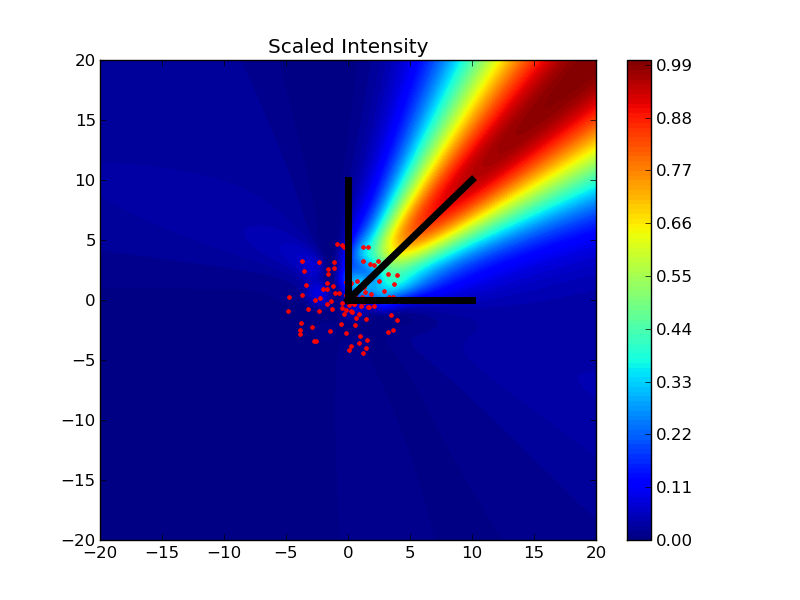
\includegraphics[width=1.0\textwidth]{phaseMatchStill.png}
   \caption{An example of how phase matching actually works.  The red dots are all emitting molecules and the black bar pointing up and the black bar pointing to the right are the k-vectors of the input beams.  The Emissions are then all added up and I've plotted the intensity, along with the addition of the two k-vectors to show they are both most definitely going in the same direction. }
	\label{fig:phaseMatached}
\end{figure}

The vertical and horizontal black bars are the input k-vectors and the skewed black bar is the phase matching direction which you can see significant intensity of light coming out of.  Red dots are the individual dipoles used in this simulation (100 in this case).

You will often hear the argument that phase matching is just a product of conservation of momentum.  You had a photon with momentum $k_1$ coming in and then another with $k_2$ coming in: of course the output will have a k-vector of $k_1 + k_2$.  That intuition will actually never lead you astray, so feel free to use it, but know that it's not physical.  When the molecule absorbs the photon, the momentum conservation happens right then and there: there's recoil in the molecule once the photon hits it.  The later-emitting dipole radiation is going out in all directions, but interfering with all the neighboring dipoles

\subsubsection{Determining the Direction of a term in the Grand Electric Field Expansion}
Phase matching comes from the imprinting of a $k$ phase on a molecule but the above derivation was done, implicitly, only considering phases applied to a bra term.  What if you care about the following term from the Grand Electric Field Expansion:
\begin{align*}
	\bra{\psi_{1+, 2-} (t)} \doublemu \ket{\psi_{1+,3+} (t)}
\end{align*}
the bra will contribute phase of $k_1 + k_3$ but the bra is less obvious.  The physics of excitation by pulse one, followed by relaxation of pulse 2 is still there, so it's counter-intuitive, but the phase is flipped from the notation in the argument of the bra.  You'll have to watch out, though, as you go out into the real world as some authors prefer the opposite convention: keeping the intuition for phases and leaving behind the intuition of + exciting and - relaxing.  Also if you ever see a thing called a double-sided Feynman diagram, they are just another tool to make sense of the Grand Electric Field Expansion\footnote{Double-sided Feynman diagrams also aid in the understanding of de-phasing when one is doing calculations which involve the density matrix of a system but we are not treating that here.}. I prefer the latter because it's more physical and intuitive in my mind.  So then in what direction does the above term radiate in?  The answer is $k_3  + k_2$.


\section{Absorption Spectra}
An absorption/emission spectrum is the most basic of spectroscopies we will cover here.  The setup in question is a light source comes into a system and excites it: only one interaction although multiple interactions will occur, as we will see, the most important interaction is just one absorption.

This process of light interaction provides lots of information about a molecule’s structure through the energy transitions allowed by the method of spectroscopy.  The method can be tuned to tell you more about electrons absorbing energy or the nucleus absorbing energy either through vibrations (Infrared/Raman spectroscopy) or the nuclear spin state through Nuclear Magnetic Resonance (NMR) spectroscopy and its variants.

The different forms of absorption spectroscopy are the oldest form of spectroscopy.  Indeed, the first absorption experiment could be said to have taken place in 1802 when Wollaston first noticed odd dark bands in sunlight he had just separated by his improved version of Newton’s prism~\cite{Wollaston}.  It turns out the gaps Wollaston observed in the spectrum were molecules between the sun and the experimenter.  Spectroscopy like that eventually proved indispensable to detecting molecules and learning about their structure.  Today there’s not a working scientist whose work doesn’t benefit from absorption spectroscopy whether they directly use it or not.

I will focus on electronic absorption but the techniques are quite interchangeable.

But what does absorption mechanistically look like?  After the system absorbs a photon, the system then proceeds to emit light.  If the incoming beam had a k-vector $k_1$ then the emission will also be in the same direction.  Mathematically this looks like this:
\begin{align}
	E_{\text{Abs}} (t) = i\frac{1}{4 \pi \epsilon_0} \frac{\omega^2}{c^2} \bra{\Psi_0 (t)} \doublemu \ket{\Psi_{1+} (t)}
\end{align}

For the basic example of a vibrational monomer, what will this signal look like?  First a little Housekeeping/definitions.  We start with a two-level system.
\begin{align}
	H_0 &= \hbar \omega_e \ket{e}\bra{e} \\
	U_0(t, \tau) &= \ket{g}\bra{g} + e^{-i \omega_e \left( t - \tau \right) } \ket{e}\bra{e}
\end{align}
but we want a vibrational coordinate on both electronic sites as well for our purposes, so we introduce one,
\begin{align}
	H_0 &=  \sum_n \hbar \omega_{\gamma}  \left(n + \frac{1}{2} \right)  \ket{n_{\gamma}}\ket{g}\bra{g} \bra{n_{\gamma}} + \sum_m \left(  \hbar \omega_{\epsilon}  \left(m + \frac{1}{2} \right) + \omega_e \right)  \ket{m_{\epsilon}} \ket{e}\bra{e} \bra{m_{\epsilon}} \\
	U_0(t, \tau) &= \sum_n e^{-i \omega_{\gamma}  \left(n+ \frac{1}{2} \right) (t - \tau) } \ket{n_{\gamma}}\ket{g}\bra{g} \bra{n_{\gamma}} + \sum_m e^{- i \left( \omega_{\epsilon}\left(m  + \frac{1}{2}\right)  +  \omega_e \right) (t - \tau) } \ket{m_{\epsilon}} \ket{e}\bra{e} \bra{m_{\epsilon}}
\end{align}
and it interacts with an electric field thusly to get the first order term
\begin{align}
	\ket{\psi_{1+}(t)} &= -\frac{i}{\hbar} \int_{-\infty}^{t}U(t, \tau) \hat{H}'_{1+} (\tau) \ket{\psi_{0}(\tau)} d\tau\\
	 &= -\frac{i}{\hbar} \int_{-\infty}^{t}U(t, \tau) E_{1+} (\tau) \hat{\mu}  e^{-i \omega_0 \tau}\ket{0_{\gamma}}\ket{g}d\tau\\
	 &= -\frac{i}{\hbar} \int_{-\infty}^{t}U(t, \tau) E_{1+} (\tau)  e^{-i \omega_0 \tau}\mu(x)\ket{0_{\gamma}}\ket{e}d\tau
\end{align}
where we now must change the vibrational basis
\begin{align}
	\ket{\psi_{1+}(t)} &= -\frac{i}{\hbar} \int_{-\infty}^{t}U(t, \tau) E_{1+} (\tau) e^{-i \omega_0 \tau}\sum_{n}\ket{n_{\epsilon}}\bra{n_{\epsilon}}\mu(x)\ket{0_{\gamma}}\ket{e}d\tau
\end{align}
where we let $\bra{n_{\epsilon}}\mu(x)\ket{0_{\gamma}} = \mu_{0}^{n}$
\begin{align}
	\ket{\psi_{1+}(t)} &= -\frac{i}{\hbar} \sum_n \int_{-\infty}^{t}U(t, \tau) E_{1+} (\tau) e^{-i \omega_0 \tau}\mu_{0}^{n}\ket{n_{\epsilon}}\ket{e}d\tau
\end{align}
and the time-evolution operator can now be applied
\begin{align}
	\ket{\psi_{1+}(t)} &= -\frac{i}{\hbar} \sum_n \mu_{0}^{n} \int_{-\infty}^{t} E_{1+} (\tau) e^{-i \omega_0 \tau}e^{-i \omega'_{e, n} (t - \tau)} \ket{n_{\epsilon}}\ket{e}d\tau
\end{align}
where $\omega'_{e, n}$ is the energy of the excited state in the $n$th vibrational level.  We simplify:
\begin{align}
	\ket{\psi_{1+}(t)} &= -\frac{i}{\hbar} \sum_n \mu_{0}^{n}  e^{-i \omega'_{e, n} t} \int_{-\infty}^{t} E_{1+} (\tau) e^{i \left( \omega'_{e, n} - \omega_0 \right) \tau} \ket{n_{\epsilon}}\ket{e}d\tau
\end{align}
If we now assume we primarily care about the time after which the pulse or perturbation has turned off, then we can extend the limit out to positive infinity  and define $\Delta \omega_{e, n} =  \omega'_{e, n} - \omega_0$
\begin{align}
	\ket{\psi_{1+}(t)} &= -\frac{i}{\hbar} \sum_n \mu_{0}^{n}  e^{-i \omega'_{e, n} t} \int_{-\infty}^{\infty} E_{1+} (\tau) e^{i \Delta \omega_{e, n}\tau} \ket{n_{\epsilon}}\ket{e}d\tau
\end{align}
Now this looks an awful lot like a Fourier transform and it is.  Now we need a specific form for the electric field envelope:
\begin{align}
	 E_{1+} (\tau) &= \frac{A}{\sqrt{2 \pi \sigma^2}} e^{-\frac{(\tau - t_1)^2}{2 \sigma^2}} e^{-i \omega_c(\tau - t_1)} \\
	 \int_{-\infty}^{\infty}  E_{1+} (\tau)  e^{i \omega t} dt &= A e^{i \omega t_1} e^{- \frac{\sigma^2}{2} \left(  \omega - \omega_c\right)^2} = \tilde{E}_{1+} (\omega)
\end{align}
which we can then put into the expression:
\begin{align}
	\ket{\psi_{1+}(t)} &= -\frac{i}{\hbar} \sum_n e^{-i \omega'_{e, n} t}  \mu_{0}^{n}   \tilde{E}_{1+} (\Delta \omega_{e, n}) \ket{n_{\epsilon}}\ket{e}
\end{align}
As a side note, this is an incredibly versatile trick.  If you ever have a perturbation $E_a(t)$ which effectively turns off at a certain time, the perturbed wavefunction will always look like a sum of all the accessible energy states multiplied by the transition dipole moment, multiplied by the amplitude of the electric field at the relevant energy level transition so long as the time you are interested in is after the perturbation turns off.  I will use that a lot going forward.

\subsubsection{2 vibrational coordinates}
What if we were to instead look at a 2-dimensional vibrational coordinate? Then we have to go back to the beginning
\begin{align}
	\ket{\psi_{1+}(t)} &= -\frac{i}{\hbar} \int_{-\infty}^{t}U(t, \tau) E_{1+} (\tau) \hat{\mu}  e^{-i \omega_0 \tau}\ket{0, 0_{\gamma}}\ket{g}d\tau\\
	 &= -\frac{i}{\hbar} \int_{-\infty}^{t}U(t, \tau) E_{1+} (\tau)  e^{-i \omega_0 \tau}\mu(x)\ket{0,0_{\gamma}}\ket{e}d\tau
\end{align}
and this time, the basis change will be more difficult.  We have to multiply in a 2D identity: $I = \sum_{n, m}\ket{n, m_{\epsilon}}\bra{n, m_{\epsilon}}$
\begin{align}
	\ket{\psi_{1+}(t)} &= -\frac{i}{\hbar} \int_{-\infty}^{t}U(t, \tau) E_{1+} (\tau)  e^{-i \omega_0 \tau}  \sum_{n, m}\ket{n, m_{\epsilon}}\bra{n, m_{\epsilon}} \mu(x)\ket{0,0_{\gamma}}\ket{e}d\tau \\
	&= -\frac{i}{\hbar} \sum_{n, m} \int_{-\infty}^{t}U(t, \tau) E_{1+} (\tau)  e^{-i \omega_0 \tau}  \ket{n, m_{\epsilon}}\mu_{0,0}^{n,m} \ket{e}d\tau
\end{align}
at this point, it's clear we will end up with an incredibly similar situation as before:
\begin{align}
	\ket{\psi_{1+}(t)} &= -\frac{i}{\hbar} \sum_{n,m} e^{-i \omega'_{e, n, m} t}  \mu_{0, 0}^{n, m}   \tilde{E}_{1+} (\Delta \omega_{e, n, m}) \ket{n, m_{\epsilon}}\ket{e}
\end{align}

\subsection{Bringing it all together}
With all the relevant perturbations collected, we return to calculating the signal.
\begin{align}
	\ket{\psi_{1+}(t)} &= -\frac{i}{\hbar} \sum_n e^{-i \omega'_{e, n} t}  \mu_{0}^{n}   \tilde{E}_{1+} (\Delta \omega_{e, n}) \ket{n_{\epsilon}}\ket{e} \\
	\ket{\psi_{0}(t)} &= e^{-i \omega'_{g, 0} t} \ket{0_{\gamma}}\ket{e} \\
	P_{\text{Abs}}(t) &= -\frac{i}{\hbar} \sum_n e^{-i \left( \omega'_{e, n} - \omega'_{g, 0} \right) t}  \mu_{0}^{*n}  \mu_{0}^{n} \tilde{E}_{1+} (\Delta \omega_{e, n}) \\
	E_{\text{Abs}}(t) &= \frac{1}{\hbar} \frac{1}{4 \pi \epsilon_0 c^2}\sum_n \left(\omega'_{e, n} - \omega'_{g, 0} \right)^2 e^{-i \left( \omega'_{e, n} - \omega'_{g, 0} \right) t}  \mu_{0}^{*n}  \mu_{0}^{n} \tilde{E}_{1+} (\Delta \omega_{e, n}) \\
	\tilde{E}_{\text{Abs}}(\omega) &= \frac{1 }{\hbar} \frac{1}{4 \pi \epsilon_0 c^2}\sum_n \left( \omega'_{e, n} - \omega'_{g, 0} \right)^2  \mu_{0}^{*n}  \mu_{0}^{n} \tilde{E}_{1+} (\Delta \omega_{e, n}) \frac{ \delta\left[ \omega -  \left( \omega'_{e, n} - \omega'_{g, 0} \right) \right] }{d\tau}\\
 	&= \frac{1 }{\hbar} \frac{1}{4 \pi \epsilon_0 c^2}\omega^2 \sum_n  \mu_{0}^{*n}  \mu_{0}^{n} \tilde{E}_{1+} (\Delta \omega_{e, n}) \frac{ \delta\left[ \omega -  \left( \omega'_{e, n} - \omega'_{g, 0} \right) \right] }{d\tau} \\
 	&= C \omega^2 \sum_n  \mu_{0}^{*n}  \mu_{0}^{n} \tilde{E}_{1+} (\Delta \omega_{e, n})  \delta\left[ \omega -  \Delta \omega_{e, n} \right]
\end{align}
As one might expect from the name absorption spectrum, we see an oscillation at all the frequency transitions from the ground state to all possible excited vibrational states.  This is tempered by the amplitude of the excitation pulse at the relevant transition energy and the dipole element, often referred to as the Franck-Condon factor $\mu_{0}^{n}  \mu_{0}^{n}$.

\subsection{Real Data}
Experimentalists will often give us the  the molar extinction constant, what do we do with that and what is it?  It's $\epsilon$ below:
\begin{align*}
	A &= c l \epsilon(\omega) = \log \left( \frac{I_0(\omega)}{I(\omega)} \right)\\
	c l \epsilon(\omega) &= \log \left( \frac{I_0(\omega)}{I_0(\omega) + \delta I(\omega)} \right)\\
	c l \epsilon(\omega) &= \log \left( \frac{1}{1 + \frac{\delta I(\omega)}{I_0(\omega)}} \right)
\end{align*}
let's then investigate this dimensionless parameter:
\begin{align*}
	\frac{\delta I(\omega)}{I_0(\omega)}
\end{align*}
but what is $\delta I (\omega)$?  Well in reality, we are putting the light source exciting the molecule into the system, at the same time that it is emitting light.  So what we're actually measuring is:
\begin{align*}
		I (\omega) &=  \left|  \tilde{E}_{1+}(\omega) +  E_{\text{abs}}(\omega) \right|^2 \\
		&= \left|  \tilde{E}_{1+}(\omega) \right|^2 + 2 \Re \left[ E_{\text{Abs}}(\omega) \tilde{E}^*_{1+}(\omega)  \right] +  \left|   E_{\text{Abs}}(\omega) \right|^2\\
		&= I_{0}(\omega) + 2 \Re \left[ E_{\text{Abs}}(\omega) \tilde{E}^*_{1+}(\omega)  \right] +  \left|   E_{\text{abs}}(\omega) \right|^2 \\
		\delta I (\omega) &= 2 \Re \left[ E_{\text{Abs}}(\omega) \tilde{E}^*_{1+}(\omega)  \right] +  \left|   E_{\text{Abs}}(\omega) \right|^2
\end{align*}
Starting with the first term using our previous model:
\begin{align*}
	\Re \left[ E_{\text{Abs}}(\omega) \tilde{E}^*_{1+}(\omega)  \right] &= \Re \left[ C \omega^2 \sum_n  \mu_{0}^{*n}  \mu_{0}^{n} \tilde{E}_{1+} (\Delta \omega_{e, n}) \delta \left[ \omega - \Delta \omega_{e, n} \right] \tilde{E}^*_{1+}(\omega)  \right] \\
	&= \Re \left[ C \omega^2 \sum_n  \mu_{0}^{*n}  \mu_{0}^{n} \delta \left[ \omega - \Delta \omega_{e, n} \right] \tilde{E}_{1+} (\Delta \omega_{e, n})  \tilde{E}^*_{1+}(\Delta \omega_{e, n})  \right]\\
	&= \Re \left[ C \omega^2 \sum_n  \mu_{0}^{*n}  \mu_{0}^{n} \delta \left[ \omega - \Delta \omega_{e, n} \right] \left| \tilde{E}_{1+} (\Delta \omega_{e, n}) \right|^2  \right] \\
	&= C \omega^2 \sum_n  \mu_{0}^{*n}  \mu_{0}^{n} \delta \left[ \omega - \Delta \omega_{e, n} \right] I_0 (\omega) = \Xi (\omega) I_0 (\omega)
\end{align*}
The delta-function doing a lot there to make the calculations simpler.  This is a cool result, here, showing that there is a dimensionless function we'll call $\Xi (\omega)$ that is multiplied by the input laser source intensity to get the first term of $\delta I$.  Now we check out the second term
\begin{align*}
	\left| E_{\text{Abs}}(\omega) \right|^2 &= \left|  C \omega^2 \sum_n  \mu_{0}^{*n}  \mu_{0}^{n} \tilde{E}_{1+} (\Delta \omega_{e, n}) \delta \left[ \omega - \Delta \omega_{e, n} \right] \right|^2 \\
	&= \left| C \omega^2 \sum_n  \mu_{0}^{*n}  \mu_{0}^{n} \delta \left[ \omega - \Delta \omega_{e, n} \right] \right|^2 I_0 \left(\omega \right)
\end{align*}
I'm about to do something a lot of people won't like... and that is to take the square of the delta function to be delta.  Close your eyes if you don't like that sort of mathematical liberty:
\begin{align*}
	\left| E_{\text{Abs}}(\omega) \right|^2 &= C^2 \omega^4 \sum_n  \left( \mu_{0}^{*n}  \mu_{0}^{n}\right)^2 \delta \left[ \omega - \Delta \omega_{e, n} \right]  I_0 \left(\omega \right) \\
	&=  \Xi^2 (\omega) I_0 (\omega)
\end{align*}
$\Xi$ has turned out to be very useful as here we see it again being squared.  We can now go back to our dimensionless intensity ratio which is:
\begin{align*}
	\frac{\delta I(\omega)}{I_0(\omega)} &=  2 \Xi(\omega) + \Xi^2 (\omega)
\end{align*}
bringing this back to the measured molar extinction coefficient
\begin{align*}
	c l \epsilon(\omega) &= \log \left( \frac{1}{1 + \frac{\delta I(\omega)}{I_0(\omega)}} \right) \\
	&= \log \left( \frac{1}{1 + 2 \Xi(\omega) + \Xi^2 (\omega) } \right)\\
	&= \log \left( \frac{1}{\left( 1 + \Xi(\omega) \right)^2 } \right) \\
	&= -2\log\left( 1 + \Xi(\omega) \right)\\
	&= -2\sum_n \sum_i (-1)^i \frac{ \left( \Xi (\omega)\right)^{i+1} }{i+1} \\
	&\approx -2 \Xi (\omega) \\
	c l \epsilon(\omega) &\approx  C \omega^2 \sum_n  \mu_{0}^{*n}  \mu_{0}^{n} \delta \left[ \omega - \Delta \omega_{e, n} \right]
\end{align*}
The last approximation is justified by noting this is essentially a series in the fine structure constant:
\begin{align*}
	C \omega^2 * \mu^2  &\propto C \omega^2 * e^2 l^2 \\
	&\propto \left(\frac{1}{4 \pi \epsilon_0 c^2 \hbar} \right) \omega^2 e^2 l^2 \\
	&= \left(\frac{e^2}{4 \pi \epsilon_0 c^2 \hbar} \right) \omega^2 l^2 \\
	&= \alpha \omega^2 l^2
\end{align*}



\section{Pump Probe Experiments}
With absorption spectroscopy, we put one laser beam, but why not put in more?  Pump Probe is what happens when we put two laser beams in and instead of measuring how much of the first beam is absorbed, we look at how much of the second beam is absorbed.  Then, because we only care about the signal which will come out in the direction of the probe beam, we have to only consider terms in the Grand Electric Field Expansion which will output in the probe direction.  There are 4 and they have names based on the physical phenomenon they are measuring.
\begin{tabular}{cccc}
Signal & Ket Interactions & Bra Interactions & Name \\
1 & pu+, pu-, pr+ & none & Ground State Bleach 1 \\
2 & pu+, pr+ & pu+ & Excited State Absorption \\
3 & pu+ & pu+, pr- & Stimulated Emission \\
4 & pr+ & pu+, pu- & Ground State Bleach 2
\end{tabular}
and then the output electric fields look like so:
\begin{align}
	E_1 (t) &=  i \bra{\psi_{0} (t)} \hat{\mu} \ket{\psi_{\text{pu+, pu-, pr+}} (t)}\\
	E_2 (t) &=  i \bra{\psi_{\text{pu+}} (t)} \hat{\mu} \ket{\psi_{\text{pu+, pr+}} (t)}\\
	E_3 (t) &=  i \bra{\psi_{\text{pu+, pr-}} (t)} \hat{\mu} \ket{\psi_{\text{pu+}} (t)}\\
	E_4 (t) &=  i \bra{\psi_{\text{pu+, pu-}} (t)} \hat{\mu} \ket{\psi_{\text{pr+}} (t)} \\
	E_{\text{pp}} (t) &= E_1(t)  + E_2(t)  + E_3(t)  + E_4(t)  \\
	S_{\text{pp}} (T) &= 2 \text{Re} \left[ \int E^*_{\text{pp}} (t) E_{\text{pr+}} (t) dt  \right]
\end{align}

\section{Higher Order Experiments}

There are many types of higher-order experiments and not terribly hard to concoct a new spectroscopy scheme.  The most common as 2-D techniques where instead of just one pump beam, there are two pump beams, and the same for the probe.  Then by scanning not just the middle gap between the pump pair and the probe pair, you also scan the two gaps between the pump/pairs.  Then by Fourier transforming the gap between the pairs, you can get a picture of the energy input and the energy output of the system under investigation.  That's just a high level explanation; I won't be going into detail as my PhD did not include much work on 2D spectroscopy.

As mentioned, you can go even higher than 4 pulses and I recently had the honor of providing a perspective for an article on a 6th order laser spectrum which I reproduce in Chapter \ref{ch:sciencePerspective}.


\section{Representations of the Nuclear Coordinate}
For the rest of this thesis, we will be very interested in forms of the transition dipole which are not just constant numbers but exist as functions.  In particular, the science I have worked on has all involved vibrational coordinate dependence of the transition dipole moment.  In order to understand how to do algebra with operators that are proportional to vibrational coordinates, it is worthwhile to understand the raising and lowering operator formulation of the Harmonic oscillator.

The Harmonic oscillator Hamiltonian looks like so:
\begin{align*}
	\hat{H} =& \frac{\hat{p}^2}{2 m} + \frac{1}{2} m \omega^2 \left(  \hat{x} - \bar{x}_0 \right)^2
\end{align*}
which has eigenstates $\ket{n}$ for which:
\begin{align}
	\hat{H} \ket{n} = \left( n \omega + \frac{1}{2} \right) \ket{n}
\end{align}
And it is useful to define operators:
\begin{align*}
	\hat{a} &= \sqrt{\frac{m \omega}{2 \hbar}} \left( \hat{x} - \bar{x}_0 + \frac{i}{m \omega} \hat{p}  \right) \\
	\hat{a}^{\dagger} &= \sqrt{\frac{m \omega}{2 \hbar}} \left( \hat{x} - \bar{x}_0 - \frac{i}{m \omega} \hat{p}  \right)
\end{align*}
such that
\begin{align}
	\hat{a}^{\dagger} \hat{a} &= \frac{m \omega}{2 \hbar} \left( \hat{x} - \bar{x}_0 - \frac{i}{m \omega} \hat{p}  \right) \left( \hat{x} - \bar{x}_0 + \frac{i}{m \omega} \hat{p}  \right) \\
	&=\frac{m \omega}{2 \hbar} \left[  \left(  \hat{x} - \bar{x}_0 \right)^2 +  \frac{1}{m^2 \omega^2} \hat{p}^2  - \frac{i}{m \omega} \left( \hat{p} \hat{x} - \hat{x} \hat{p} \right) \right]
\end{align}
we know, however, that:
\begin{align}
	[\hat{x}, \hat{p}] = \hat{x} \hat{p}  - \hat{p} \hat{x} = i \hbar
\end{align}\begin{align}
	\hat{a}^{\dagger} \hat{a} &=\frac{m \omega}{2 \hbar} \left[  \left(  \hat{x} - \bar{x}_0 \right)^2 +  \frac{1}{m^2 \omega^2} \hat{p}^2  +\frac{i}{m \omega} i \hbar \right] \\
	&=\frac{m \omega}{2 \hbar} \left[  \left(  \hat{x} - \bar{x}_0 \right)^2 +  \frac{1}{m^2 \omega^2} \hat{p}^2  -\frac{\hbar}{m \omega} \right]\\
	&= \frac{m \omega}{2 \hbar}  \left(  \hat{x} - \bar{x}_0 \right)^2 +  \frac{m \omega}{2 \hbar} \frac{1}{m^2 \omega^2} \hat{p}^2  -\frac{m \omega}{2 \hbar}  \frac{\hbar}{m \omega} \\
	&= \frac{m \omega}{2 \hbar}  \left(  \hat{x} - \bar{x}_0 \right)^2 +  \frac{1}{2 \hbar} \frac{1}{m \omega} \hat{p}^2  -\frac{1}{2 }
\end{align}
we now note that with a little manipulation:
\begin{align}
	\hat{H} = \hbar \omega \left(  \hat{a}^{\dagger} \hat{a} + \frac{1}{2}\right)
\end{align}
So we define the product of those two operators in that manner as the number operator:
\begin{align}
	\hat{N} &= \hat{a}^{\dagger} \hat{a}
\end{align}
because when you act it on an eigenstate:
\begin{align}
	\hat{N} \ket{n} &= n \ket{n}
\end{align}
We can now note that because the ladder operators are made of position and momentum operators that they themselves will have commutators as well
\begin{align}
	\left[\hat{a}^{\dagger}, \hat{a} \right] &= 1 \\
	\left[\hat{N}, \hat{a} \right] &= - \hat{a}\\
	\left[\hat{N}, \hat{a}^{\dagger} \right] &= \hat{a}^{\dagger}
\end{align}
Now we might ask what happens when we act the number operator on an eigenstate for which the operator $\hat{a}^{\dagger}$ has been appended:
\begin{align*}
	\hat{N}\hat{a}^{\dagger} \ket{n} &= \left( \hat{N}\hat{a}^{\dagger}  + \hat{a}^{\dagger} \hat{N}- \hat{a}^{\dagger} \hat{N}\right) \ket{n}\\
	&= \left( [N, \hat{a}^{\dagger}] + \hat{a}^{\dagger}  \hat{N} \right) \ket{n}\\
	&= \left(  \hat{a}^{\dagger}  + \hat{a}^{\dagger}  \hat{N} \right) \ket{n}\\
	&= \left(  1  + n  \right)\hat{a}^{\dagger} \ket{n}
\end{align*}
implying that the operator $\hat{a}^{\dagger}$ adds a quanta of energy. Similarly:
\begin{align*}
	\hat{N}\hat{a} \ket{n} &= \left( \hat{N}\hat{a}  + \hat{a}^{} \hat{N}- \hat{a}^{} \hat{N}\right) \ket{n}\\
	&= \left( [N, \hat{a}^{}] + \hat{a}^{}  \hat{N} \right) \ket{n}\\
	&= \left( - \hat{a}^{}  + \hat{a}^{}  \hat{N} \right) \ket{n}\\
	&= \left(   n - 1  \right)\hat{a}^{} \ket{n}
\end{align*}
and that $\hat{a}$ operator takes away a quanta.  But what exactly does an application of one of these operators look like?
\begin{align*}
	\hat{a} \ket{n}&= \sqrt{n} \ket{n-1} \\
	\hat{a}^{\dagger} \ket{n} &= \sqrt{n+1} \ket{n+1}
\end{align*}
Because I don't feel like deriving them right now.
\subsubsection{Position and Momentum Operators}
We can take the ladder operators and turn them into position and momentum operators,
\begin{align*}
	\hat{a} &= \sqrt{\frac{m \omega}{2 \hbar}} \left( \hat{x} - \bar{x}_0 + \frac{i}{m \omega} \hat{p}  \right) \\
	\hat{a}^{\dagger} &= \sqrt{\frac{m \omega}{2 \hbar}} \left( \hat{x} - \bar{x}_0 - \frac{i}{m \omega} \hat{p}  \right)
\end{align*}
say we add them together:
\begin{align*}
	\hat{a}^{\dagger} + \hat{a} &=2 \sqrt{\frac{m \omega}{2 \hbar}}  \left( \hat{x} - \bar{x}_0 \right)   \\
	\left( \hat{x} - \bar{x}_0 \right) &= \sqrt{\frac{\hbar}{2 m \omega}} \left(  \hat{a}^{\dagger} + \hat{a}  \right)
\end{align*}
which gives us as a final answer:
\begin{align}
	\hat{x} &= \bar{x}_0 + \sqrt{\frac{\hbar}{2 m \omega}} \left(  \hat{a}^{\dagger} + \hat{a}  \right)
\end{align}
similarly when we subtract the ladder operators:
\begin{align*}
	\hat{a}^{\dagger} - \hat{a} &=-2 \sqrt{\frac{m \omega}{2 \hbar}}  \frac{i}{m \omega} \hat{p} \\
	&=- i\sqrt{\frac{2}{\hbar m \omega}}  \hat{p}
\end{align*}
giving us:
\begin{align}
	 \hat{p} &= i\sqrt{\frac{\hbar m \omega}{2}} \left( \hat{a}^{\dagger} - \hat{a} \right)
\end{align}



\subsubsection{The Huang-Rhys Parameter}
Say we want a dimensionless quantity that will tell us something about the difference between two potential energy wells.  This would mean we have two Hamiltonians:
\begin{align*}
	\hat{H}_{\gamma} =& \frac{\hat{p}^2}{2 m_{\gamma}} + \frac{1}{2} m_{\gamma} \omega_{\gamma}^2 \left(  \hat{x} - \bar{x}_{\gamma} \right)^2 + E_{\gamma}
\end{align*}
and
\begin{align*}
	\hat{H}_{\epsilon} =& \frac{\hat{p}^2}{2 m_{\epsilon}} + \frac{1}{2} m_{\epsilon} \omega_{\epsilon}^2 \left(  \hat{x} - \bar{x}_{\epsilon} \right)^2 + E_{\epsilon}
\end{align*}
We could look at the value of one potential energy surface(ignoring any constant offset)  at the difference between the two center points:
\begin{align*}
	V_{\epsilon} (\bar{x}_{\gamma} ) &= \frac{1}{2} m_{\epsilon} \omega_{\epsilon}^2 \left(  \Delta \bar{x} \right)^2 \\
	\Delta \bar{x} &= \bar{x}_{\epsilon} - \bar{x}_{\gamma}
\end{align*}
this is called the reorganization energy, because it is the amount of energy that would be ``lost'' or ``gained'' to go from one equilibrium point to another.  This is not, however, dimensionless but it will be if we divide it by a quanta of energy:
\begin{align*}
	\frac{V_{\epsilon} (\bar{x}_{\gamma} ) }{\hbar \omega_{\epsilon}} &= \frac{m_{\epsilon }\omega_{\epsilon}}{2 \hbar} \left(  \Delta \bar{x} \right)^2 = S
\end{align*}
Which is called the Huang-Rhys Parameter or $S$ in our notation and characterizes the change in equilibrium position between two harmonic potential energy wells.  Now, at this point, you should be asking:  Isn't this an equally valid measure of the difference between two potential energy wells?
\begin{align*}
	\frac{V_{\gamma} (\bar{x}_{\epsilon} ) }{\hbar \omega_{\gamma}} &= \frac{m_{\gamma }\omega_{\gamma}}{2 \hbar} \left(  \Delta \bar{x} \right)^2 = S
\end{align*}
and I think you would be right but I do not know how to resolve this paradox...  What you COULD do is note that these dimensionless parameters suggest the existence of dimensionless  units of measurement of distance.
\begin{align*}
	S_{\epsilon}&= \frac{m_{\epsilon }\omega_{\epsilon}}{2 \hbar} \left(  \Delta \bar{x} \right)^2 \\
	&= \frac{1}{2}\left( \sqrt{\frac{m_{\epsilon }\omega_{\epsilon}}{ \hbar} } \Delta \bar{x} \right)^2
\end{align*}
and then just take the square of the difference between the two dimensionless locations of the center of the potential energy wells:
\begin{align*}
	S &= \frac{1}{2}\left( \sqrt{\frac{m_{\epsilon }\omega_{\epsilon}}{ \hbar} }  \bar{x}_{\epsilon}  - \sqrt{\frac{m_{\gamma }\omega_{\gamma}}{ \hbar} }  \bar{x}_{\gamma}  \right)^2
\end{align*}
but apparently the proper convention (citation needed) is
\begin{align*}
	S &= \frac{m_{\epsilon} \omega_{\epsilon} m_{\gamma }\omega_{\gamma }\left(  \Delta \bar{x} \right)^2 }{m_{\epsilon}  \omega_{\epsilon} +  m_{\gamma } \omega_{\gamma}}
\end{align*}
Which would reduce to the previous formula is both the masses and both the frequencies were the same.

\subsection{What Happens when you apply a ladder operator to the wrong eigenstate?}
For the purposes of this thesis, we will often encounter two different potential energy wells on the same molecule (one for its ground state, $\gamma$,  and the other for its excited state, $\epsilon$).  Does it matter if we apply a ladder operator from $\gamma$ to $\epsilon$?  Let's see.
\begin{align*}
	\hat{a}^{\dagger}_{\gamma} \ket{n_{\epsilon}}
\end{align*}
but we only know for sure how the operator works in its own basis so we transform to that basis using the identity operator $\sum_i \ket{i_{\gamma}}\bra{i_{\gamma}}$ and my shorthand for the frank-Condon factor $\braket{a_{\gamma}|b_{\epsilon}} = O_a^b$:
\begin{align*}
	\hat{a}^{\dagger}_{\gamma} \ket{n_{\epsilon}} &= \hat{a}^{\dagger}_{\gamma} \sum_{i} O_{i}^{n}\ket{i_{\gamma}} \\
	&= \sum_{i} O_{i}^{n} \hat{a}^{\dagger}_{\gamma} \ket{i_{\gamma}}\\
	&= \sum_{i} O_{i}^{n} \sqrt{i + 1} \ket{i + 1_{\gamma}}
\end{align*}
Now what if we bring it back into the original basis?
\begin{align*}
	\hat{a}^{\dagger}_{\gamma} \ket{n_{\epsilon}} &= \sum_{i,j} O_{i}^{n} O_{i + 1}^{j}  \sqrt{i + 1} \ket{j_{\epsilon}}
\end{align*}
If we had mistakenly assumed the ladder operators were the same, we would have gotten:
\begin{align*}
	\hat{a}^{\dagger}_{\gamma} \ket{n_{\epsilon}} \neq \sqrt{n+1} \ket{n+1_{\epsilon}}
\end{align*}
But what is the amplitude that really ends up in the $\ket{n+1_{\epsilon}}$ state?
\begin{align*}
	\bra{n+1_{\epsilon}}\hat{a}^{\dagger}_{\gamma} \ket{n_{\epsilon}} &= \sum_{i,j} O_{i}^{n} O_{i + 1}^{j}  \sqrt{i + 1}\delta_{j,n+1} \\
	 &= \sum_{i} O_{i}^{n} O_{i + 1}^{n+1}  \sqrt{i + 1}
\end{align*}
So one must be very, very careful to apply the correct ladder operators to the correct state.



\section{Nuclear Structure of the Electronic Transition Dipole Moment and the Condon Approximation}

One of the more common transition dipole moments to see looks like this,
\begin{align}
	 \doublemu = \vec{\mu}_0  \left( \ket{e}\bra{g} + \ket{g}\bra{e} \right)
\end{align}
where $\vec{\mu}_0 $ is just a constant vector which does not depend on any other variable.  Edward Condon in 1928 made with surprisingly little justification the above approximation that the electronic transition dipole did not depend on the nuclear position at all.  But that should seem wrong, because shouldn't a molecule be more likely to transition when it's in a nuclear configuration that is more similar to the state it's not in?  There is no reason that instead of $\vec{\mu}_0$, we can substitute an arbitrary function of the nuclear position $\vec{\mu} (\vec{R})$.  For the purposes of illustration, we will always collapse this object into a scalar which is only a function of one coordinate $\mu (x)$.  We also then expand it into a polynomial basis,
\begin{align}
	\mu(x) &= \mu_0  \sum_i \kappa_i x^i
\end{align}
but we know from above that this can be expressed in terms of creation and annihilation operators,
\begin{align}
	\mu(x) &= \mu_0  \sum_i c_i \left(\hat{a} + \hat{a}^{\dagger}\right)^i
\end{align}
To keep things as simple as possible in analytic expressions, we normally will only work with the linear correction.
\begin{align}
	\mu(x) &= \mu_0  + \mu' x
\end{align}
\subsection{Different Potential Energy Wells}
If we take the above operator, we realize we need it to be able to act it on two potential energy wells $\gamma$ and $\epsilon$ with their own sets of eigenstates: $\{ \ket{n_{\gamma}}\}$ and $\{ \ket{n_{\epsilon}}\}$.  What will that operator look like in terms of the ladder operators for each well?  We'll start with the $\gamma$ state:
\begin{align}
	\mu(x) &= \mu_0  + \mu' \left(  \bar{x}_{\gamma}+ \sqrt{\frac{\hbar}{2 m_{\gamma} \omega_{\gamma}}} \left(  \hat{a}_{\gamma}^{\dagger} + \hat{a}_{\gamma}  \right)\right) \\
	&= \left( \mu_0  + \mu'   \bar{x}_{\gamma} \right)  + \mu'  \sqrt{\frac{\hbar}{2 m_{\gamma} \omega_{\gamma}}} \left(  \hat{a}_{\gamma}^{\dagger} + \hat{a}_{\gamma}  \right)
\end{align}
and the epsilon will look frightfully similar:
\begin{align}
	\mu(x) 	&= \left( \mu_0  + \mu'   \bar{x}_{\epsilon} \right)  + \mu'  \sqrt{\frac{\hbar}{2 m_{\epsilon} \omega_{\epsilon}}} \left(  \hat{a}_{\epsilon}^{\dagger} + \hat{a}_{\epsilon}  \right)
\end{align}
but we want them to look neat, so we define a few more variables:
\begin{align}
	\mu(x) &= \bar{\mu}_{\gamma} + \mu'_{\gamma }  \left(  \hat{a}_{\gamma}^{\dagger} + \hat{a}_{\gamma}  \right) \\
	&= \bar{\mu}_{\epsilon} + \mu'_{\epsilon }  \left(  \hat{a}_{\epsilon}^{\dagger} + \hat{a}_{\epsilon}  \right) \\
	\bar{\mu}_{\gamma}  &= \left( \mu_0  + \mu'   \bar{x}_{\gamma} \right) \\
	\bar{\mu}_{\gamma}  &= \left( \mu_0  + \mu'   \bar{x}_{\epsilon} \right) \\
	\mu'_{\gamma } &=  \mu'  \sqrt{\frac{\hbar}{2 m_{\gamma} \omega_{\gamma}}} \\
	\mu'_{\epsilon } &=  \mu'  \sqrt{\frac{\hbar}{2 m_{\epsilon} \omega_{\epsilon}}}
\end{align}
Then if we wanted to make the operator exceedingly simple in one basis, $\gamma$, what would the constants look like for $\epsilon$?
\begin{align*}
	\mu(x) &= 1+ c \left(  \hat{a}_{\gamma}^{\dagger} + \hat{a}_{\gamma}  \right) \\
	\bar{\mu}_{\gamma} &= 1 =  \mu_0  + \mu'   \bar{x}_{\gamma}  \\
	\mu'_{\gamma }  &= c = \mu'  \sqrt{\frac{\hbar}{2 m_{\gamma} \omega_{\gamma}}}\\
	\mu(x) &= d+ c_{\epsilon} \left(  \hat{a}_{\epsilon}^{\dagger} + \hat{a}_{\epsilon}  \right) \\
	\bar{\mu}_{\epsilon} &= d =  \mu_0  + \mu'   \bar{x}_{\epsilon}  \\
	\mu'_{\epsilon }  &= c_{\epsilon} = \mu'  \sqrt{\frac{\hbar}{2 m_{\epsilon} \omega_{\epsilon}}}\\
\end{align*}
we can now do some algebra:
\begin{align*}
	1 - d &= \mu'   \bar{x}_{\gamma} - \mu'   \bar{x}_{\epsilon}  \\
	d &= 1 - \mu' \left(  \bar{x}_{\epsilon}  -  \bar{x}_{\gamma}  \right)
\end{align*}
or in terms of c:
\begin{align*}
	d &= 1 - c \sqrt{\frac{2 m_{\gamma} \omega_{\gamma}}{\hbar}}  \Delta x
\end{align*}
and some more algebra:
\begin{align*}
	\frac{c_{\epsilon}}{c}  &=  \sqrt{\frac{\hbar}{2 m_{\epsilon} \omega_{\epsilon}}}  \sqrt{\frac {2 m_{\gamma} \omega_{\gamma}}{\hbar}} \\
	\frac{c_{\epsilon}}{c}  &=  \sqrt{\frac{m_{\gamma} \omega_{\gamma}}{m_{\epsilon} \omega_{\epsilon}}}\\
	c_{\epsilon}  &=  c \sqrt{\frac{m_{\gamma} \omega_{\gamma}}{m_{\epsilon} \omega_{\epsilon}}}
\end{align*}

\subsubsection{Getting a dimensionless $c$}
We initially defined the transition dipole function as
\begin{align}
	\mu(x) &= \mu_0  + \mu' x
\end{align}
but suppose we want a dimensionless number to describe the slope, let's construct one:
\begin{align}
	\mu(x) &= \mu_0  \left( 1 + \frac{\mu'}{\mu_0} x \right) \\
	&= \mu_0  \left( 1 + \Delta x \frac{\mu'}{\mu_0} \frac{x}{\Delta x} \right)
\end{align}
where $\Delta x = \bar{x}_{\epsilon} - \bar{x}_{\gamma}$.  We can then define $\lambda = \Delta x \frac{\mu'}{\mu_0} $ as a completely dimensionless way to describe how much variation in the transition dipole a wavepacket would experience when traversing the potential energy wells
\begin{align}
	\mu(x) &=  \mu_0  \left( 1 + \lambda \frac{x}{\Delta x} \right)
\end{align}

\subsubsection{A Natural Estimate of $\lambda$}
Looking at the paper ``Vibronic effects in the spectroscopy and dynamics of C-phycocyanin''~\cite{photosyntheticKappa}, and, specifically, figure 9c, the black line represents the author's worst (most non-Condon) transition dipole that they calculated.  The transition dipole is roughly linear, with a value of -3 Debye at x=0 and decreasing .5 Debye in .5 distance units giving a slope of 1 Debye per dimensionless distance unit .  They quote the dimensionless displacement as being .4 which we can then use to extract an estimate for $\lambda$ in a real system.
\begin{align*}
	\mu (x) &\approx -3 - \frac{.5}{.5} x \\
	&= -3 \left(  1 + \frac{x}{3}\right)\\
	&= -3 \left(  1 + \frac{x}{3} \frac{d}{d}\right) \\
	&= -3 \left(  1 +  \frac{d}{3} \frac{x}{d}\right) \\
	\lambda &= \frac{d}{3} = \frac{.4}{3} = .1\bar{3}
\end{align*}



% \section{Physical Basis of the Condon Approximation}
% The dipole of a molecule is merely the charge-weighted position of charges:
% \begin{align*}
% 	\vec{\mu} &= \sum_i q_i r_i
% \end{align*}
% and it describes the distribution of charge.  It might make sense to separate the variables into nuclear and electronic:
% \begin{align*}
% 	\vec{\mu} &= \sum_l Q_l R_l + \sum_{\lambda} q _{\lambda} * r_{\lambda}
% \end{align*}
%
% \begin{align*}
% 	\mu_{l,\lambda \leftarrow a, \alpha} = \int  \phi^*_l (R_n) \psi^*_{\lambda} (r_e) r_e \phi_l (R_n) \psi_{\lambda} (r_e) dr_e
% \end{align*}
%
% TODO: FLESH THIS OUT OR DELETE?
